\section{问题四：技术演进分析与前沿预测}

\subsection{口径统一}

前三问以交叉熵损失为对象，本问转向多维 Benchmark 得分，因此必须先统一四个口径，否则后续分解无从谈起。

\textbf{能力度量。} 采用 C1 榜单的综合得分 \texttt{Average}（六项任务 IFEval、BBH、MATH Lvl 5、GPQA、MUSR、MMLU-PRO 的等权平均），缺失任务不自动按剩余项平均冒充完整六维分数。

\textbf{逐任务聚合。} 题面要求至少完成一项逐任务聚合。本文对 C8 的 1958 份 JSON 解析 BBH 的 24 个子任务，做\textbf{宏平均}（子任务等权）并以\textbf{题量加权平均}作对照，共成功解析 1859 个模型、4 份损坏。只聚合叶子任务，避免了父子任务重复计数。与 C1 的 BBH 列对比发现二者存在稳定的仿射关系：

\begin{equation}
\text{C1}_{\mathrm{BBH}}=-36.78+1.3249\times\text{C8}_{\text{宏平均}},
\qquad \rho=0.9979 .
\end{equation}

这说明\textbf{C1 的 BBH 列并非原始正确率，而是经过归一化（很可能是随机猜测校正）后的分数}，直接把 C8 的 \texttt{acc\_norm} 乘 100 替代榜单分是错的。这一核对确认了本文使用 C1 \texttt{Average} 作为能力度量的合理性。

\textbf{时间轴。} 以 C1 的提交日期为主，C2 的 Epoch AI 发布日期仅作敏感性对照，不混用。样本覆盖 2024-06-08 至 2025-03-13，分析截止日 $t_0$ 取 2025-03-13。

\textbf{开源筛选。} 严格口径要求 C4 的 \texttt{Open model weights?} 为 Yes（802 个模型），宽松口径要求榜单 Hub License 非空（2\,810 个模型）。题面要求预测开源模型的前沿，故主预测使用宽松口径的前沿基准 $S_0=37.70$；严格口径的前沿为 36.26，两者相差 1.44 分。无法判定开放性者进入未知组，不自动归类。

\textbf{模型类型。} 按 C1 的 \texttt{Type} 列区分预训练模型（3\,858 个）与对话/微调模型（718 个），在回归中作为哑变量。

\subsection{C4 元数据匹配}

题面要求使用 C4 的算力、数据量、开源权重等字段。C4 采用 Epoch AI 的自有命名（如 ``Llama 3.1-8B''），与榜单的 ``org/model'' 命名差异很大，直接同名匹配覆盖率仅 2.4\%。本文设计了分层匹配规则：

\begin{itemize}[leftmargin=2em,itemsep=2pt]
\item \textbf{high}：规范化短名（去机构前缀、去非字母数字、转小写）完全相同，107 个；
\item \textbf{medium}：一方是另一方的前缀（处理 \texttt{-Chat}、\texttt{-32K}、\texttt{-Instruct} 等后缀）且参数量比在 $[0.95,1.05]$ 内，660 个；
\item \textbf{low}：前缀关系且参数量比在 $[0.9,1.11]$ 内，43 个（仅作审计，不进主分析）。
\end{itemize}

总覆盖率升至 \textbf{17.7\%}（810/4576）。同时限制 C4 只取 Language 域、且发布日期不晚于 $t_0$，以避免使用未来信息。近 3\,800 个未匹配模型在元数据相关分析中显式排除，并在结果表中标注样本量。

\subsection{Loss--Benchmark 桥接}

前三问的结论建立在交叉熵损失上，要转成能力必须建立桥接。题面要求按可比性等级区分使用。本文对 C6 的 75 个模型按 \texttt{Loss\_Comparability} 分层拟合

\begin{equation}
S=a-bL,\qquad b\ge0,
\end{equation}

结果见表~\ref{tab:q4_bridge} 与图~\ref{fig:q4_bridge}。

\begin{table}[htbp]
\centering
\caption{Loss--Benchmark 桥接拟合（按可比性分层）}
\label{tab:q4_bridge}
\small
\begin{tabular}{l|l|r|r|r|r}
\toprule
\textbf{数据集} & \textbf{可比性等级} & \textbf{点数} & \textbf{$a$} & \textbf{$b$} & \textbf{$R^2$} \\
\midrule
\multirow{2}{*}{C6 扩展} & High（同模型同验证集） & 7 & 7.672 & $-0.882$ & 0.158 \\
                          & Medium（不同验证集，近似） & 68 & 61.434 & $-19.185$ & 0.252 \\
\midrule
\multirow{2}{*}{C5 原始} & High & 7 & 7.672 & $-0.882$ & 0.158 \\
                          & Medium & 36 & 48.929 & $-14.529$ & 0.240 \\
\bottomrule
\end{tabular}
\end{table}

\begin{figure}[htbp]
\centering
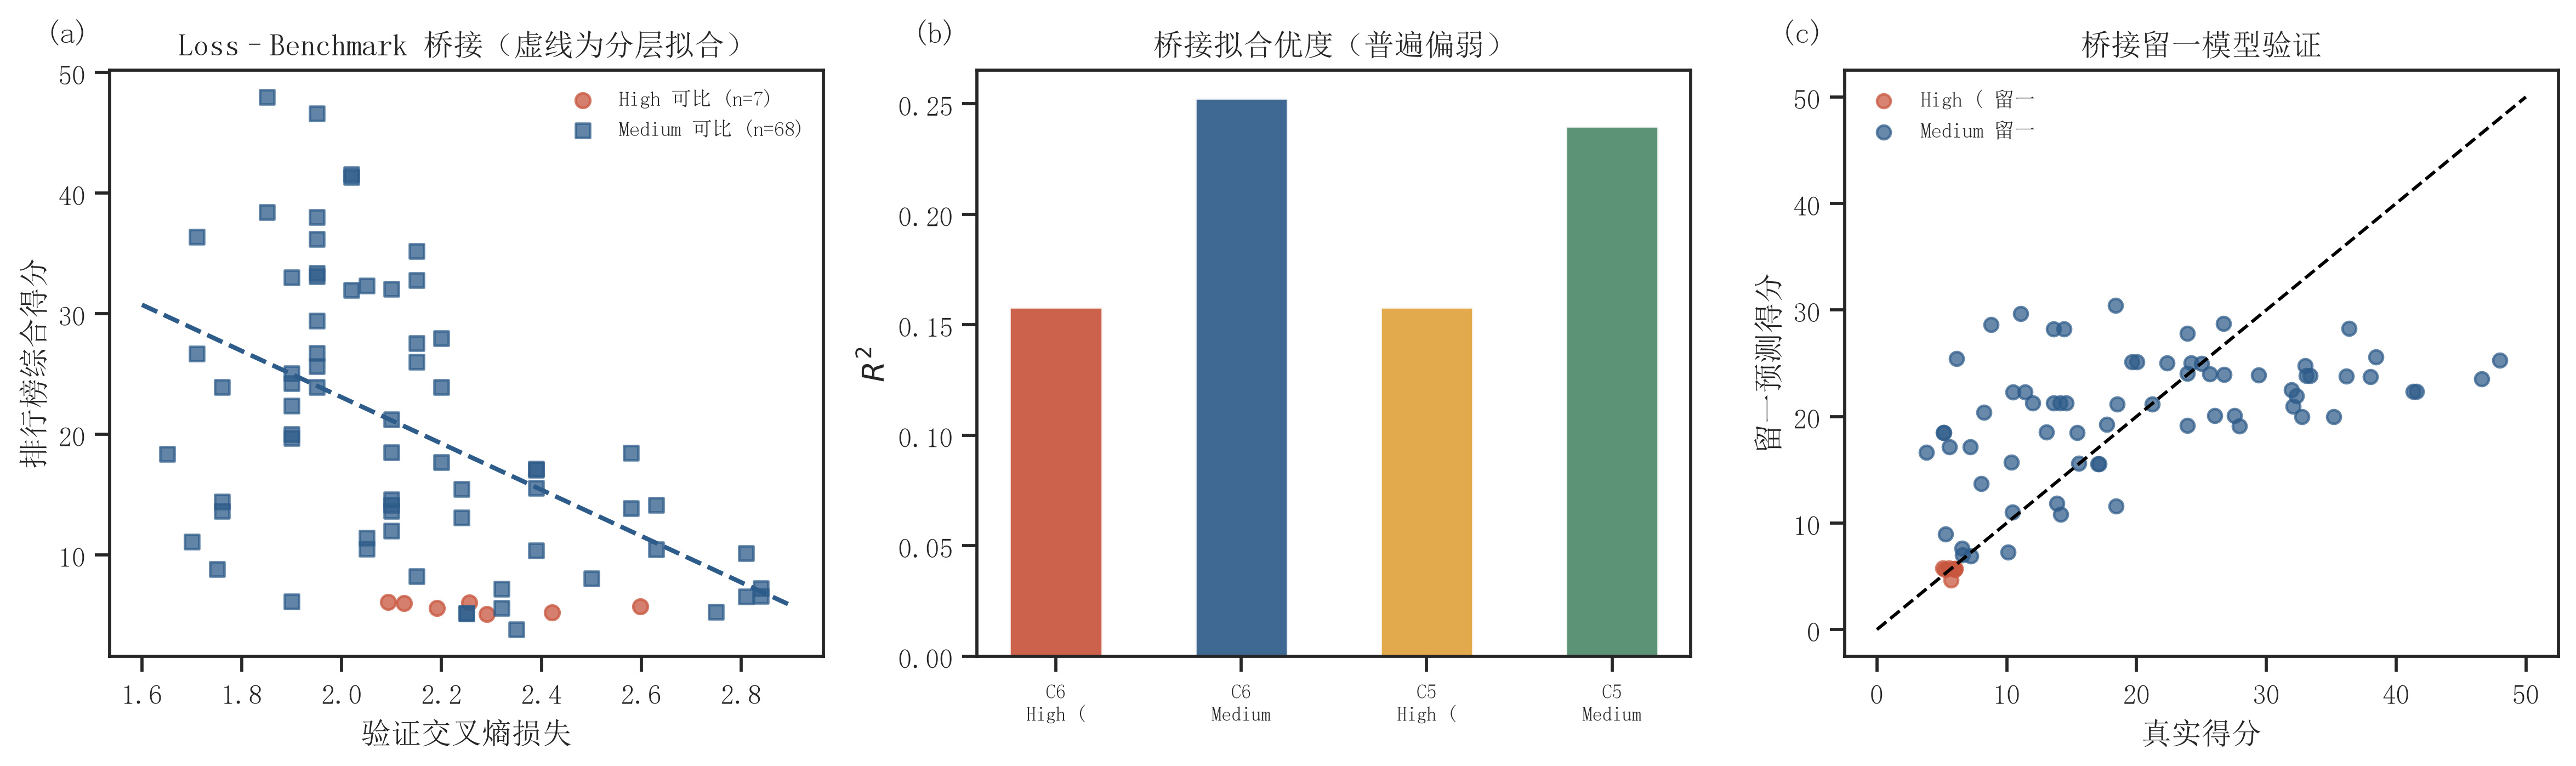
\includegraphics[width=0.95\textwidth]{figures/fig_q4_bridge.png}
\caption{桥接拟合与留一验证}
\label{fig:q4_bridge}
\end{figure}

\textbf{桥接质量很差，这是本文必须如实报告的核心局限。} 高可比组只有 7 个点（全部是 Pythia 系列，且 $D$ 固定在 299.9B），$R^2$ 仅 0.158；中可比组 68 个点，$R^2$ 也只有 0.252。留一模型验证的 MAE 为 7.34 分、RMSE 为 9.59 分。图~\ref{fig:q4_bridge}(a) 直观显示，同一损失水平下的榜单得分离散度极大——这是因为不同模型族的 tokenizer、训练数据与对齐方法差异，使``损失→能力''并非单值映射。

因此本文的立场是：\textbf{桥接只用于把损失的变化量近似折算成能力的变化趋势，不用于绝对水平预测}；所有涉及桥接的结论都在预测区间中计入这一误差。这与题面``讨论映射误差对结论的影响''的要求一致。

\subsection{能力模型与贡献分解}

\subsubsection{模型比较}

本文比较了 5 个能力模型，均以综合得分 $S$ 为因变量：

\begin{table}[htbp]
\centering
\caption{能力模型比较（因变量：C1 综合得分）}
\label{tab:q4_model}
\small
\begin{tabular}{l|r|r|r|r}
\toprule
\textbf{模型} & \textbf{样本数} & \textbf{$R^2$} & \textbf{调整 $R^2$} & \textbf{RMSE} \\
\midrule
M1: $\log N+t+\text{type}$ & 4\,561 & 0.465 & 0.464 & 7.90 \\
M2: $\log C+t+\text{type}$ & 627 & 0.485 & 0.482 & 7.72 \\
M3: $\log N+\log C+t+\text{type}$ & 627 & 0.527 & 0.524 & 7.39 \\
M4: $\log C+t+\text{type}+\text{open}$ & 595 & 0.497 & 0.493 & 7.68 \\
M5: $\log C+t+\text{type}$（高置信匹配） & 595 & 0.490 & 0.487 & 7.73 \\
\bottomrule
\end{tabular}
\end{table}

M1 覆盖最广（4\,561 个模型）且只用榜单自带参数量，作为\textbf{主模型}用于分解：

\begin{equation}
S=13.70+14.334\log_{10}N+12.846\,t+1.732\,\text{chat}.
\label{eq:q4_main}
\end{equation}

系数解读：参数量每增加 10 倍约提升 14.3 分；控制参数量与类型后，\textbf{时间趋势为每年 +12.85 分}；对话微调模型平均比同规模预训练模型高 1.73 分。M3 同时放入 $\log N$ 与 $\log C$ 后拟合最好，但二者高度相关（$C\approx6ND$），系数不可分别解释，故不作主模型。

\subsubsection{贡献分解}

题面要求分离规模扩张与非规模技术进步的贡献。直接用季度平均能力做分解会被组成变化污染——本文数据确实显示季度平均 $\log_{10}N$ 从 0.944 降到 0.757（因为提交的小模型越来越多）。因此主分解建立在\textbf{固定组成子集}（$\ge$7B 的预训练模型，组成相对稳定）上：

\begin{equation}
\Delta S_{\text{scale}}=b_N\,\Delta\log_{10}N,\qquad
\Delta S_{\text{non-scale}}=r\,\Delta t,\qquad
\Delta S_{\text{resid}}=\Delta S-\Delta S_{\text{scale}}-\Delta S_{\text{non-scale}} .
\end{equation}

由于模型对对数变量是线性的，两种因素更新顺序给出完全相同的贡献（顺序差为 0），无需再做顺序平均；这一点已单独验证并记录。

\begin{table}[htbp]
\centering
\caption{贡献分解（固定组成子集：$\ge$7B 预训练模型）}
\label{tab:q4_dec}
\small
\begin{tabular}{l|r|r|r|r|r}
\toprule
\textbf{季度} & \textbf{$\Delta S$} & \textbf{规模贡献} & \textbf{非规模贡献} & \textbf{未解释} & \textbf{规模占比} \\
\midrule
2024Q2$\to$2024Q3 & 3.169 & $-0.291$ & $+3.236$ & $+0.225$ & $-9.2\%$ \\
2024Q3$\to$2024Q4 & 5.228 & $-0.268$ & $+3.236$ & $+2.260$ & $-5.1\%$ \\
2024Q4$\to$2025Q1 & 1.133 & $-0.356$ & $+3.165$ & $-1.676$ & $-31.4\%$ \\
\midrule
\textbf{合计} & \textbf{9.530} & $\mathbf{-0.916}$ & $\mathbf{+9.636}$ & $+0.810$ & $\mathbf{-9.6\%}$ \\
\bottomrule
\end{tabular}
\end{table}

\begin{figure}[htbp]
\centering
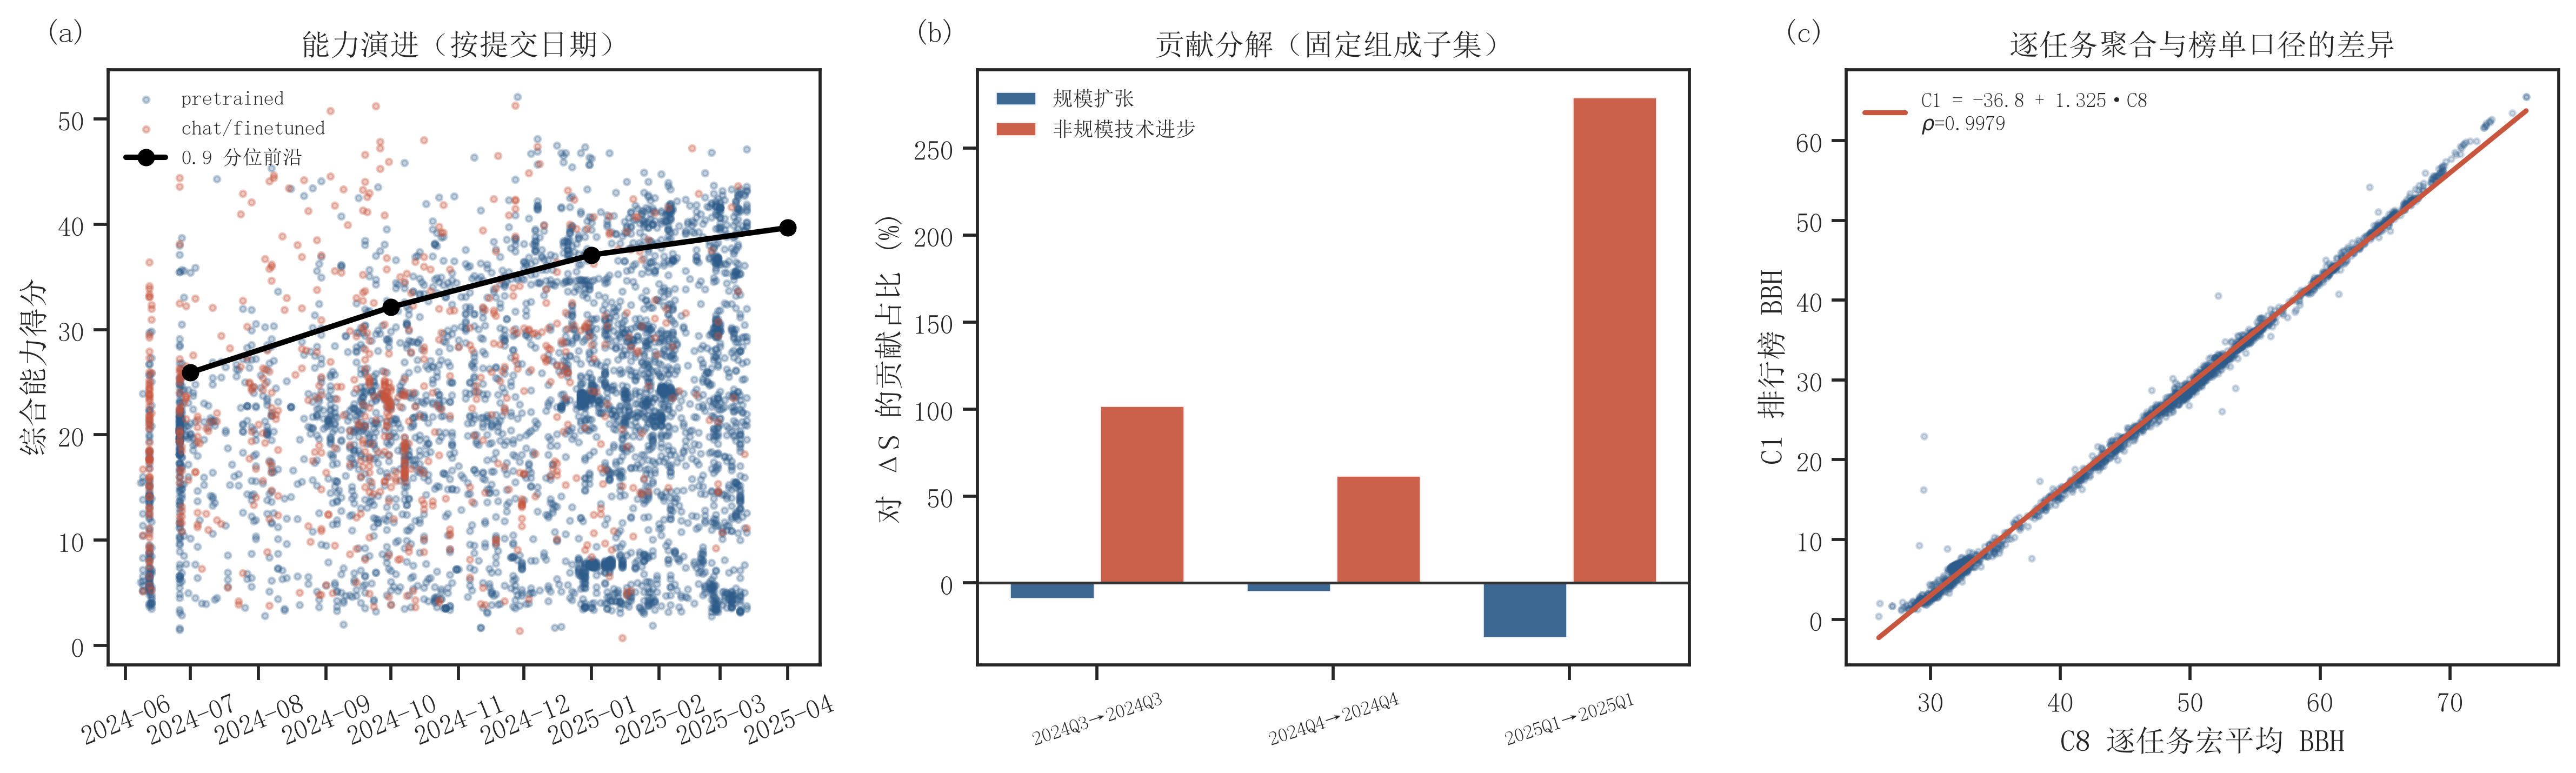
\includegraphics[width=0.95\textwidth]{figures/fig_q4_timeline.png}
\caption{能力演进时序与贡献分解}
\label{fig:q4_time}
\end{figure}

\textbf{核心结论}：在这段窗口内，能力提升 9.53 分中规模项为 $-0.92$ 分（$-9.6\%$），非规模技术进步为 $+9.64$ 分（$101.1\%$），未解释部分仅 8.5\%。也就是说，\textbf{能力增长几乎全部来自数据工程、对齐方法与架构改进等非规模因素，而前沿模型的参数量在这一时期并未增大}——固定组成子集的平均 $\log_{10}N$ 在三段区间内均为负贡献。这与题面引用的``8B 小模型胜过 GPT-4o''的现象在方向上一致。

需要如实说明三点边界：（1）该分解的是\textbf{模型预测变化}而非全部观测变化，未解释的 8.5\% 包含组成变化与遗漏因素；（2）时间项 $r$ 只表示``控制规模与类型后的剩余趋势''，\textbf{不构成因果识别}，它还可能包含评测口径变化、数据污染、后训练算力增加等遗漏因素；（3）分位数前沿口径的分解未解释比例高达 62\%，因为前沿模型的参数量波动更大，故\textbf{以固定组成口径为主报告}。

\subsection{前沿预测}

\subsubsection{算力增长率}

预测需要未来算力路径。C1$\cap$C4 匹配子集的时间跨度仅 0.76 年，不足以估计趋势，故本文改用 C4 全量 Language 域历史（2019-01 至 2025-03，558 个模型）的前沿训练算力做 0.9 分位回归，得

\begin{equation}
g=0.628\ \text{dex/年}\quad(\text{即前沿算力约每年 } \times4.2).
\end{equation}

需要说明，逐年最大值口径给出 0.480 dex/年，与分位回归的 0.628 存在差异，反映估计的不稳定性；本文取二者的中位数并\textbf{在情景中覆盖这一不确定性}，而不是声称已精确测得增长率。

\subsubsection{最优路径上的能力增长}

在算力最优配置下，由问题三的解析解可得 $N^\ast\propto C^{\beta/(\alpha+\beta)}$、$D^\ast\propto C^{\alpha/(\alpha+\beta)}$，代入 $\alpha=0.340$、$\beta=0.280$ 得份额 $w_N=0.452$、$w_D=0.548$。于是未来能力的预测式为

\begin{equation}
S(t)=S_0+\left(b_N w_N+r/g\right)\cdot g\,(t-t_0)+r\,(t-t_0),
\end{equation}

即规模路径贡献 $b_Nw_N g\Delta t$、非规模趋势贡献 $r\Delta t$。三档情景取 $g$、$0.5g$、$0.1g$，分别对应``增长延续''``增长放缓''与``算力近乎不变''。参数不确定性用对模型重采样 400 次的 bootstrap 传播。

\begin{table}[htbp]
\centering
\caption{开源模型能力前沿预测（$t_0$=2025-03-13，$S_0$=37.70）}
\label{tab:q4_forecast}
\small
\begin{tabular}{l|r|r|r|r|r}
\toprule
\textbf{算力情景} & \textbf{月份} & \textbf{规模贡献} & \textbf{非规模贡献} & \textbf{前沿预测} & \textbf{95\% bootstrap 区间} \\
\midrule
\multirow{2}{*}{增长延续（$g$）} & 12 & $+4.06$ & $+12.85$ & \textbf{54.61} & $[52.80,\ 55.64]$ \\
                                  & 24 & $+8.13$ & $+25.69$ & \textbf{71.52} & $[68.61,\ 73.69]$ \\
\midrule
\multirow{2}{*}{增长放缓（$0.5g$）} & 12 & $+2.03$ & $+12.85$ & \textbf{52.57} & $[50.81,\ 53.56]$ \\
                                    & 24 & $+4.06$ & $+25.69$ & \textbf{67.45} & $[64.65,\ 69.57]$ \\
\midrule
\multirow{2}{*}{算力近乎不变（$0.1g$）} & 12 & $+0.41$ & $+12.85$ & \textbf{50.95} & $[49.25,\ 51.91]$ \\
                                        & 24 & $+0.81$ & $+25.69$ & \textbf{64.20} & $[61.42,\ 66.21]$ \\
\bottomrule
\end{tabular}
\end{table}

\begin{figure}[htbp]
\centering
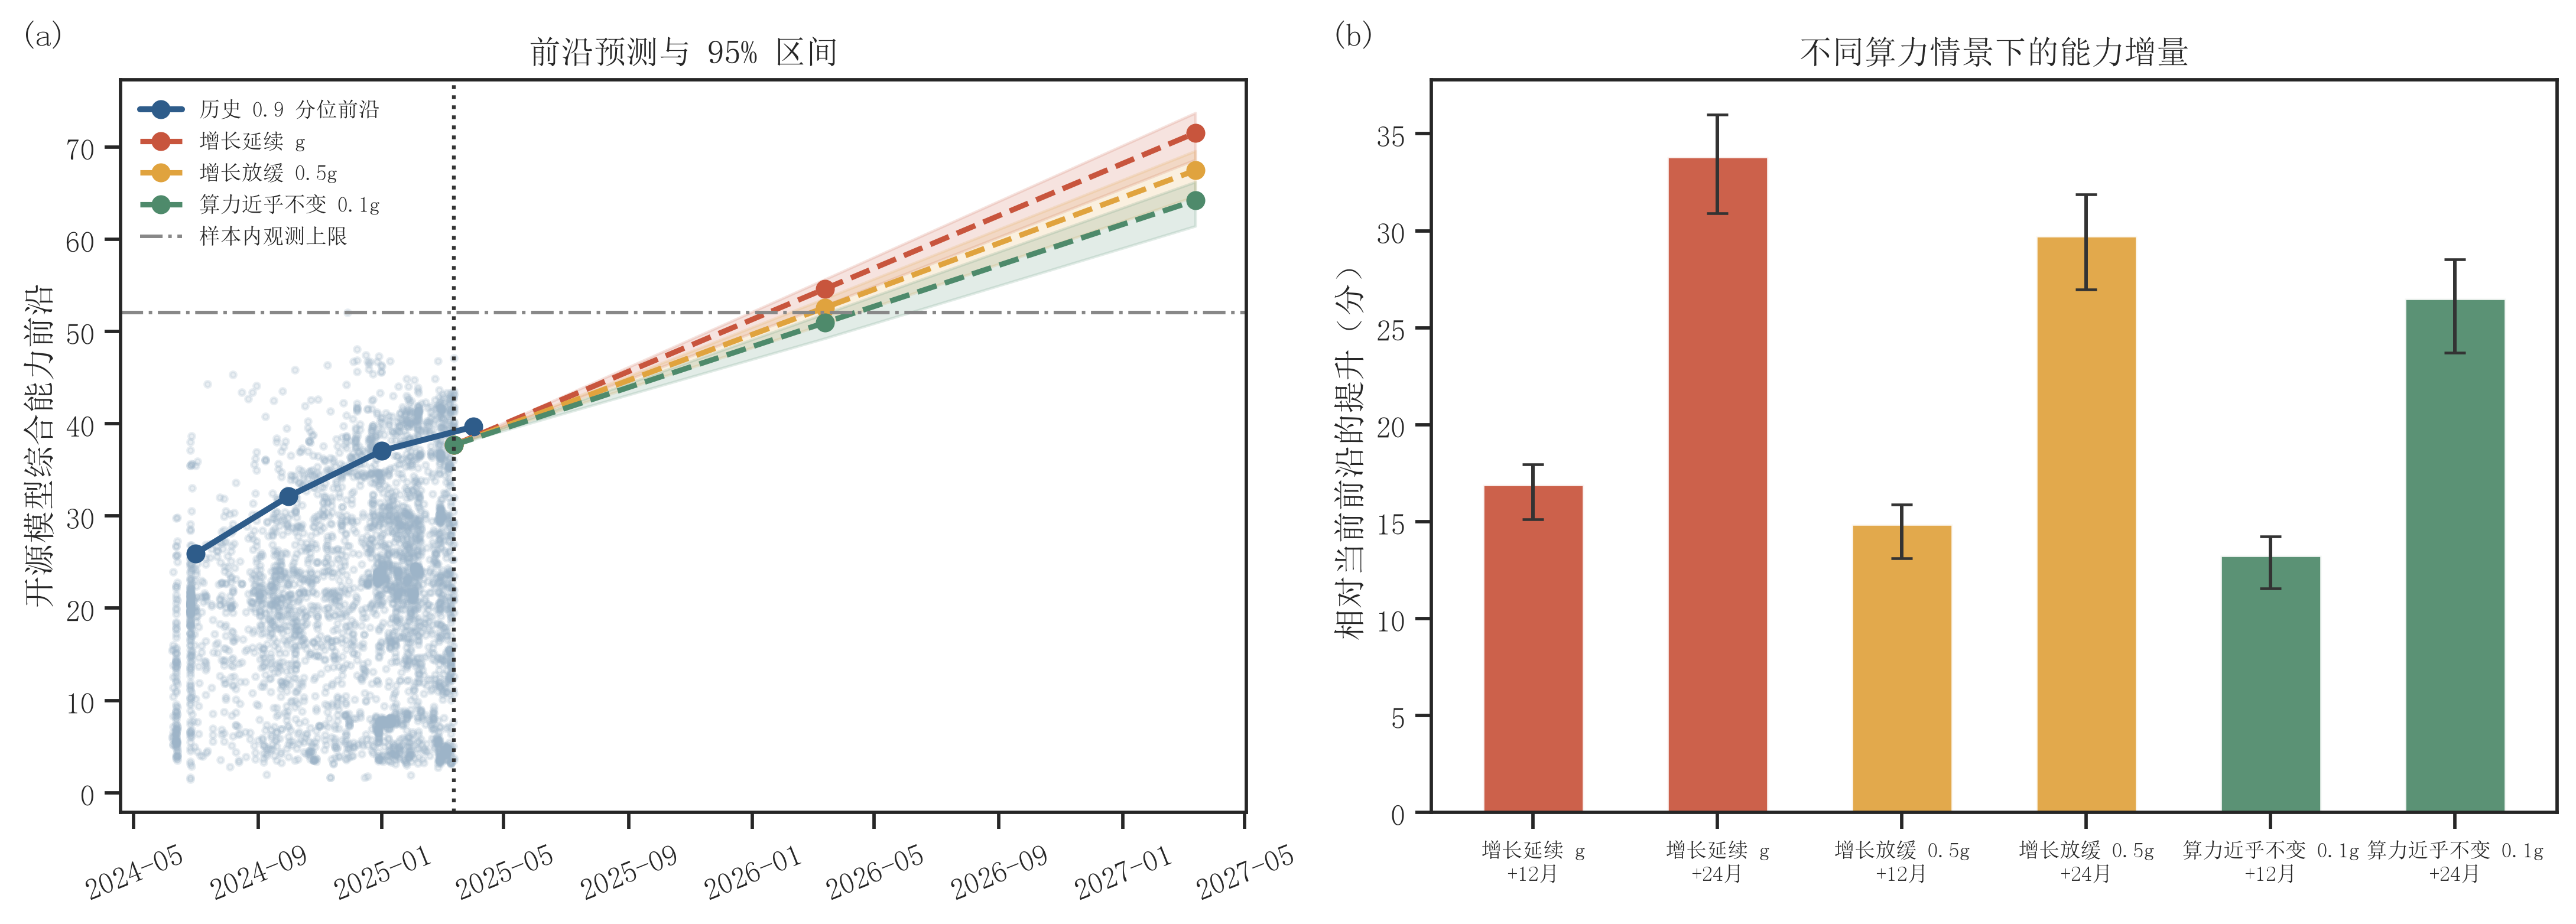
\includegraphics[width=0.95\textwidth]{figures/fig_q4_forecast.png}
\caption{前沿预测与算力情景对比}
\label{fig:q4_fc}
\end{figure}

\textbf{结果解读。} 12 个月后开源模型能力前沿预计达 50.9$\sim$54.6 分，24 个月后达 64.2$\sim$71.5 分。一个值得注意的结论是：\textbf{三档算力情景的差异远小于时间趋势本身的贡献}——即便算力增长降到十分之一，24 个月后的预测仍有 64.2 分，而增长延续也只到 71.5 分。这直接来自\ref{tab:q4_dec}节的分解结论：能力增长主要不靠算力堆叠。这一结论与问题三``质量投入存在启动预算、非规模因素更关键''的发现相互印证。

\subsubsection{饱和警示与外推边界}

必须显著标注一个边界：样本内综合得分的最大值为 \textbf{52.08} 分（99.9 分位 48.04），而 24 个月的预测值 64.2$\sim$71.5 分\textbf{全部越过该上限}。这说明线性时间趋势外推在长跨度上不可持续——榜单存在实际可达上限，且趋势项 $r$ 不可能永远保持每年 12.85 分。

因此表~\ref{tab:q4_forecast} 应读作\textbf{``按现有趋势的上界估计''，不是可信的点预测}。12 个月的预测（50.9$\sim$54.6）仅略微越过上限，可信度相对较高；24 个月的预测则明显属于外推，其价值在于给出量级与情景对比，而非精确数值。

另一方面，未来最高分还取决于参评模型的数量——提交的模型越多，出现的最高分越高。本文不建模这一数量效应，因此采用\textbf{高分位数前沿}（0.9 分位）而非``未来一定出现的最高分''，符合题面的表述要求。

\subsubsection{回测}

用时间滚动切分做回测：在每个历史截止点重新拟合，用其后 90 天的数据评估。

\begin{table}[htbp]
\centering
\caption{时间滚动回测（训练用过去，评估用未来 90 天）}
\label{tab:q4_backtest}
\small
\begin{tabular}{l|r|r|r|r|r}
\toprule
\textbf{截止点} & \textbf{训练样本} & \textbf{测试样本} & \textbf{RMSE} & \textbf{MAE} & \textbf{预测均值/真实均值} \\
\midrule
2024-10-01 & 1\,282 & 1\,316 & 8.20 & 6.51 & 22.28 / 22.52 \\
2024-11-01 & 1\,714 & 1\,765 & 7.81 & 6.09 & 22.31 / 22.46 \\
2024-12-01 & 2\,088 & 2\,131 & 8.29 & 6.41 & 23.99 / 23.13 \\
2025-01-01 & 2\,659 & 1\,902 & 9.09 & 6.94 & 25.76 / 22.78 \\
\bottomrule
\end{tabular}
\end{table}

四个截止点的 RMSE 在 7.8$\sim$9.1 分之间，均值预测与真实均值接近（偏差在 $-2.98\sim+0.86$ 分）。最后一个截止点的预测偏高 2.98 分，提示当模型组成快速变化时（该窗口内大量小模型涌入）预测会失准。回测样本量有限（仅 4 个截止点），\textbf{该结果反映的是量级而非精确的预测精度}。
